\chapter*{Introduction}
\addcontentsline{toc}{chapter}{Introduction}

Imagine, for a moment, that you are transported in time to 14th-century Europe. It is Sunday, and mass is
starting. The tall ceilings of the impressive church were built so to bring you closer to God. The stained glass windows
let through just enough light so that it is not completely dark. The scent of incens pervades the air. Everything in the environment around
you reminds you that you are taking part in a sacred ritual. Listen to the priest; when he recites the prayers, his speech just say them.
Instead, the entire text is intoned on a single note, except for the slightly inflected ends of clauses. 
Sometimes, the choir replaces the priest, singing more elaborate melodies. The words they are singing are Latin, but even 
if you do not understand them, you know what their purpose is: to celebrate the deity. Their voices echo in the stone church, creating an
otherwordly experience.

What you are hearing is called \emph{Gregorian chant}, one of the oldest preserved types of music. It has been central to the cultural development
of most of Europe, as it is a part of the Roman-catholic tradition. Figure \ref{fig:chant_manuscripts} shows an example of four chants the original manuscripts.
\footnote{\url{http://www.ksbm.oeaw.ac.at/images/AT/5000/AT5000-1011/AT5000-1011\_1v.jpg}}\footnote{\url{http://www.uni-regensburg.de/Fakultaeten/phil\_Fak\_I/Musikwissenschaft/cantus/microfilm/copenhagen/vol3/images/008.jpg}}\footnote{\url{http://manuscripta.at/diglit/AT5000-589/09}}\footnote{\url{https://gallica.bnf.fr/ark:/12148/btv1b10033588d/f5.image}} as they are found in
the original manuscripts. The chant in the upper right corner uses notation which is not dissimilar from contemporary musical notation,
while the chant in the lower right image only uses memory aids also called \emph{neumes} without the exact pitch. This highlights the differences
between the ways chant was recorded over the centuries (see Section \ref{section:notation}).

\begin{figure}[h]
\centering
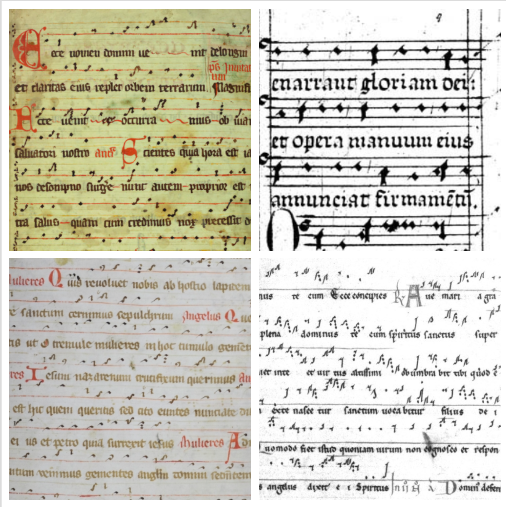
\includegraphics{chant_manuscripts}
\caption{An example of chants as inscribed in manuscripts.}
\label{fig:chant_manuscripts}
\end{figure}

Gregorian chant is a widely researched topic of study, partly thanks to the substantial amount of available sources. However, traditional
musicology is limited by the constraints of human perception of individual researchers; it is infeasible to study extremely large numbers of chants by hand. This is where
Digital Humanities come into play. Digitalization of large corpora of Gregorian chant enables researchers to draw conclusions
supported by much more data than a human could ever examine: there are hundreds of thousands of entries in collaborative chant databases.

Nevertheless, contemporary Gregorian chant research still lacks software tools that would facilitate the study of chant repertoire. An example
of an important problem is chant's historical and geographical development. Throughout the 
centuries, the tradition spread accross Europe, while always changing a small part of it. This has led to many variations of the same
chants existing at the same time. Knowing how exactly the changes came into place could shed light on many open questions in the history of 
European culture. However, no tools are currently available to e.g. compare and visualize the relationship between groups of chants; musicologists
are limited to tedious manual typesetting.

\textbf{The aim of this thesis is to create a tool that musicologists could use to answer questions about chant origin and evolution.} We do this by employing
well-known algorithms for \emph{multiple sequence alignment} (MSA) from bioinformatics.

Once the idea is proposed, it is almost immediately obvious that
biological and musical sequences share features which warrant using the same methods on both. As opposed to other sequence comparison techniques, such as edit
distance, MSA algorithms do not need any assumptions about the length of chants or other characteristics, which is why they are suitable
for the study of chant.

The tool, available online\footnote{\url{https://github.com/kszabova/rhythmify_frontend/tree/bc_final}}\footnote{\url{https://github.com/kszabova/rhythmify_backend/tree/bc_final}},
provides the ability to align a a potentially large and diverse set of chants in multiple ways, each of which has slightly different uses. One important
implication of the tool is that it makes the discovery contrafacta (chants with the same melody but different lyrics) and transpositions
(chants with the same melody but shifted by an interval) across large repertoires easy.

However, the purpose of this thesis is not to conduct experiments. It is merely a tool for musicologists who possess
the knowledge needed to select the appropriate data so that previously infeasible discoveries can be made.

